%\renewcommand\thesection{A.\arabic{section}}
%\renewcommand\thefigure{A-\arabic{figure}}   
%\renewcommand\thetable{A-\arabic{table}}   

\chapter{Appendix} \label{ch:Appendix}


\section*{Visual Results}
\subsection[]{Correlation Difference Matrix}
\label{A:corr_matrix}

\begin{figure}[h]
	\centering
	\begin{subfigure}{0.3\textwidth}
		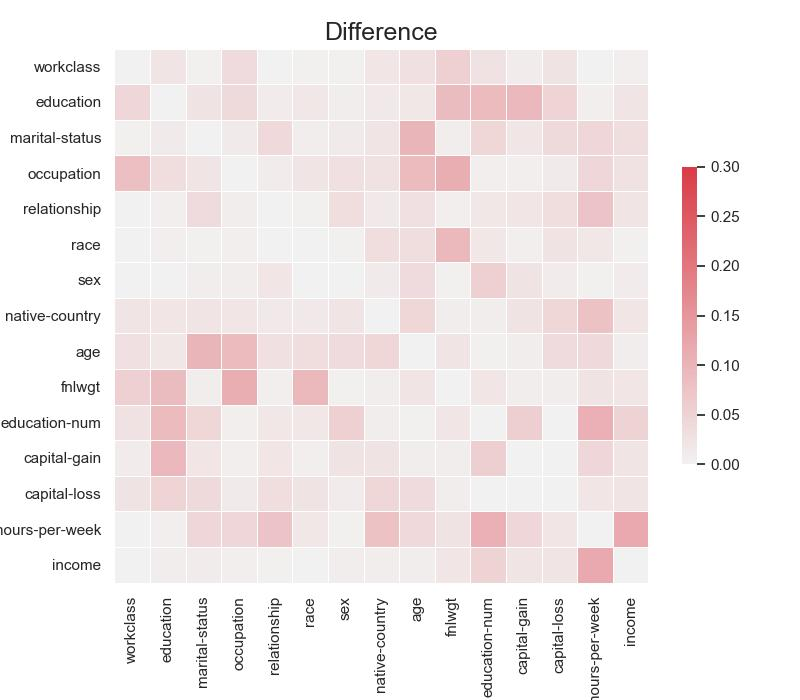
\includegraphics[width=\textwidth]{images/correlation_difference/ctabgan_simTune.jpg}
		\caption{CTABGAN$^s_q$}

	\end{subfigure}
    \begin{subfigure}{0.3\textwidth}
        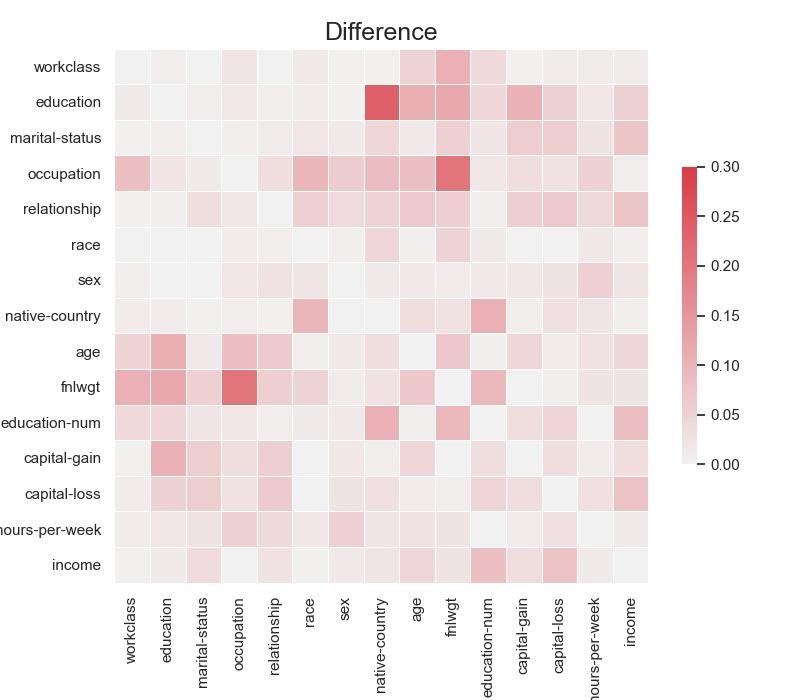
\includegraphics[width=\textwidth]{images/correlation_difference/tvae_simTune.jpg}
        \caption{TVAE$^s$}

    \end{subfigure}
	\begin{subfigure}{0.3\textwidth}
		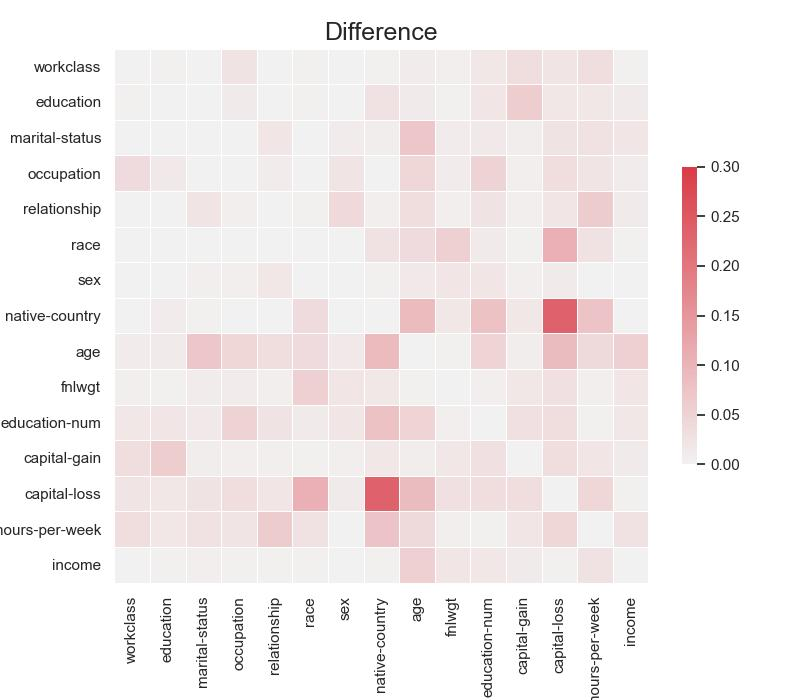
\includegraphics[width=\textwidth]{images/correlation_difference/tab-ddpm-bgm-simTune.jpg}
		\caption{TabDDPM-BGM$^{s}_q$}

	\end{subfigure}
    \begin{subfigure}{0.3\textwidth}
        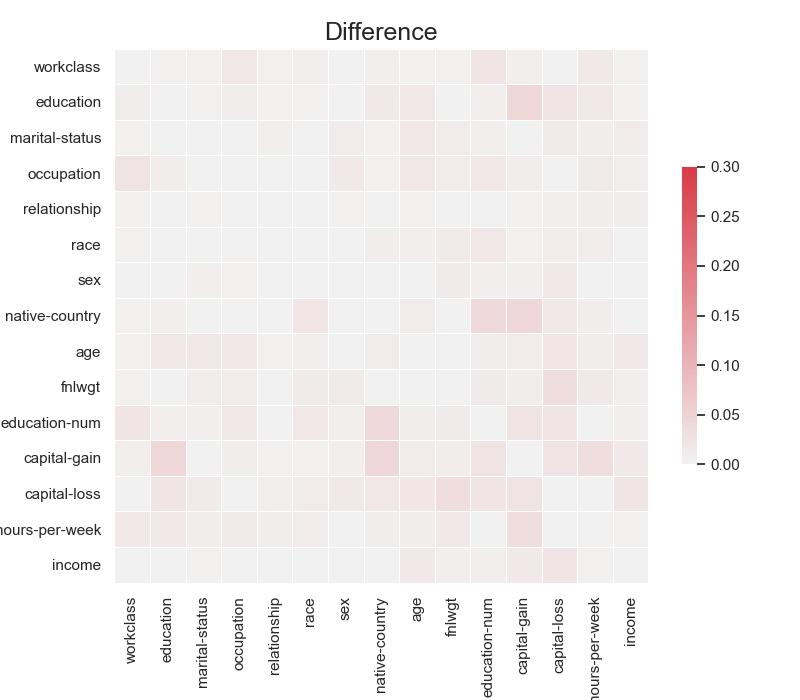
\includegraphics[width=\textwidth]{images/correlation_difference/tab-ddpm-bgm-simTune-minmax.jpg}
        \caption{TabDDPM-BGM$^{s}_m$}

    \end{subfigure}
	\begin{subfigure}{0.3\textwidth}
		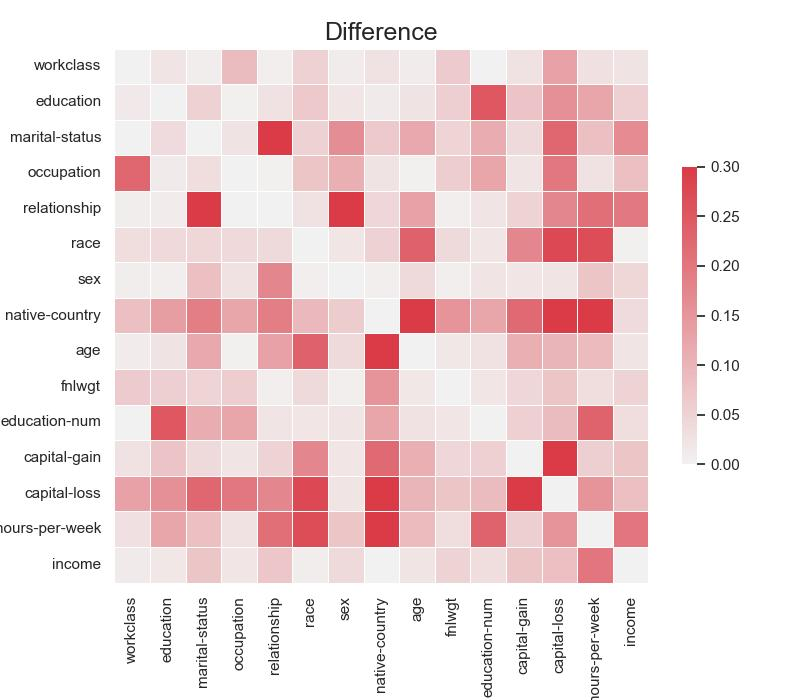
\includegraphics[width=\textwidth]{images/correlation_difference/tab-ddpm-ft-simTune.jpg}
		\caption{TabDDPM-FT$^{s}_q$}

    \end{subfigure}
    \caption{Correlation difference matrix for different model versions}

\end{figure}

\subsection[]{Principle Component Analysis}
\label{A:pca}

\begin{figure}[h]
	\centering
	\begin{subfigure}{0.3\textwidth}
		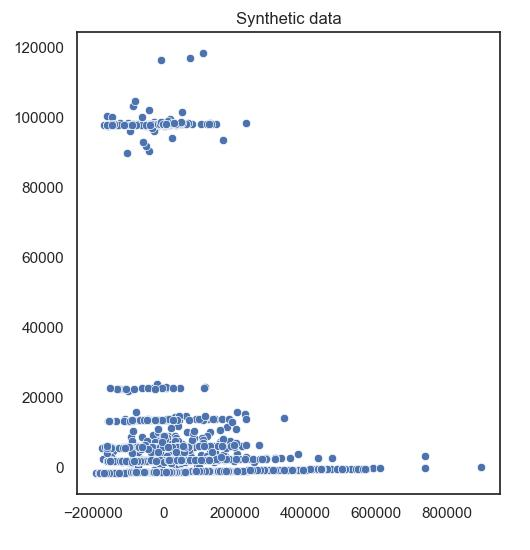
\includegraphics[width=\textwidth]{images/pca/ctabgan_simTune.jpg}
		\caption{CTABGAN$^s$}
	\end{subfigure}
    \begin{subfigure}{0.3\textwidth}
        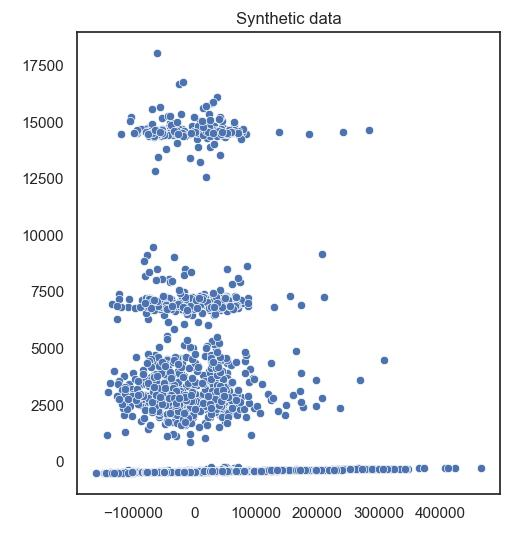
\includegraphics[width=\textwidth]{images/pca/tvae_simTune.jpg}
        \caption{TVAE$^s$}
    \end{subfigure}
	\begin{subfigure}{0.3\textwidth}
		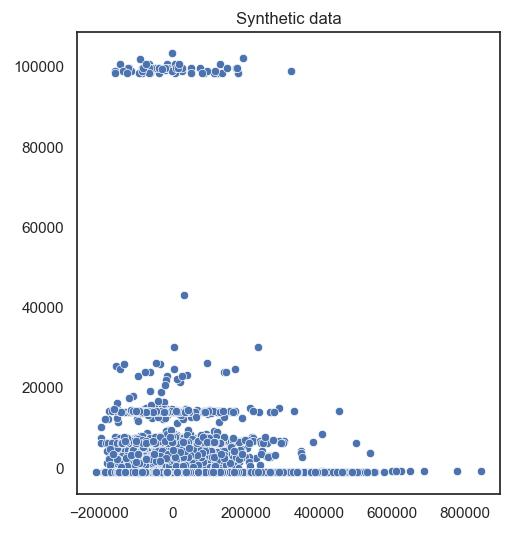
\includegraphics[width=\textwidth]{images/pca/tab-ddpm-bgm-simTune.jpg}
		\caption{TabDDPM-BGM$^{s}_q$}
	\end{subfigure}
	\begin{subfigure}{0.3\textwidth}
		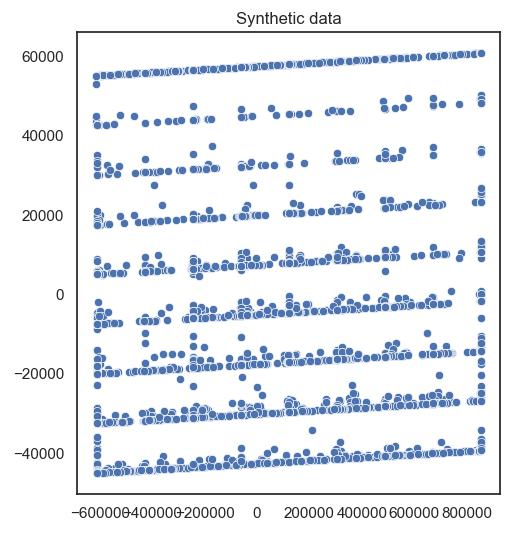
\includegraphics[width=\textwidth]{images/pca/tab-ddpm-ft-simTune.jpg}
		\caption{TabDDPM-FT$^{s}_q$}
    \end{subfigure}
	\begin{subfigure}{0.3\textwidth}
		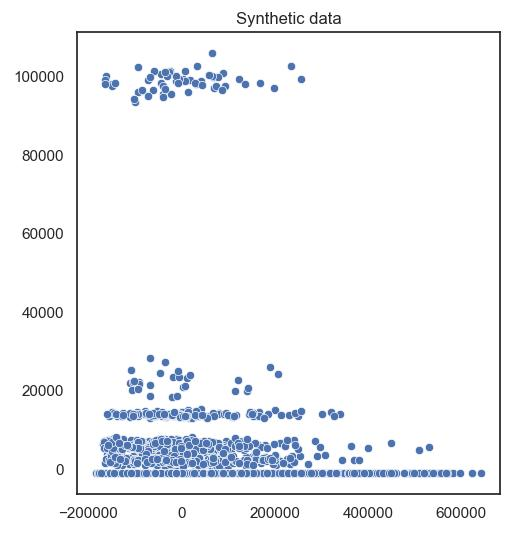
\includegraphics[width=\textwidth]{images/pca/tab-ddpm-bgm-simTune-minmax.jpg}
		\caption{TabDDPM-BGM$^{s}_m$}
		\label{fig_a:pca_TabDDPMBM}
    \end{subfigure}
    \caption{Principle Component Analysisfor different model versions}
    \label{fig_a:pca_diff}
\end{figure}



